\section{Proposed Methodology}
\label{sec:methodology}
Our machine learning algorithm is required to predict the global routing pattern of a design. Thus, it needs to be trained to create an accurate predictive model. For the purpose of training, certain features need to be extracted from designs that have already undergone global routing. Along with these features, post-routing congestion information for each edge need to be extracted. Two matrices, one containing these features and another populated with the congestion information act as input and output values required to train the machine learning model. 

We use NTHU-Route 2.0 \cite{NTHU} as the platform to implement our routability model. Since the congestion in the NTHU router is calculated using an edge-based perspective, all the features of the design are observed using a similar approach. 

\subsection{Routing Feature Extraction}
\begin{itemize}
\item \textbf{First-degree pins}. First degree pins are pins closest to an edge and are deemed to have a significant impact on the probability of the routing wire to cross-over the chosen edge, thus altering its congestion value. \Cref{fig:fdpin} depicts a visual representation of this feature. This feature provides a metric for the proximity or vicinity of pins with respect to an edge. To route a first-degree pin, at least one of the four edges surrounding that pin will be crossed by the wire.

\begin{figure}[tb!]
    \centering
    \subfloat[]{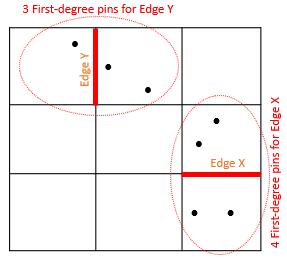
\includegraphics[width=.48\linewidth]{fdpin}  \label{fig:fdpin}}
    \subfloat[]{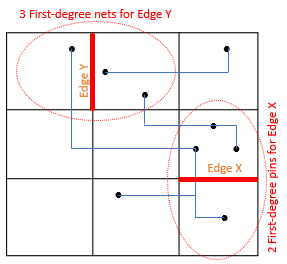
\includegraphics[width=.48\linewidth]{fdnet}  \label{fig:fdnet}}
    \caption{Examples of (a) first degree pins; (b) first degree nets.}
\end{figure}

\item \textbf{First-degree nets}. A tile can contain various pins which belong to different nets. Different pins in a tile can be a part of the same net or part of different nets. The first-degree nets of an edge are the nets that cross-over the space enclosed by either of the two tiles that the chosen edge is a part of, \Cref{fig:fdnet}  gives an example of this feature. 

\item \textbf{Pin density}. This ``density'' feature gives information regarding the number of pins per unit area. Pin density for a chosen edge is given by the number of first-degree pins divided by twice the tile area i.e., area of both tiles the edge is a part of. Pin density helps to give information of how congested the pins are within a tile which directly translates to a higher probability for the tile's corresponding edges to be used for routing. A higher pin density means that the edges of this tile can mostly be used to route pins within that tile. This deems the edges unroutable for wire connecting other tiles and thus a detour must be made. 

\item \textbf{RSMT-aware two-pin-pair usage}. This ``usage'' feature represents in the evaluation of the most appropriate path for global routing based on a probabilistic model. The router initially creates multi-pin net Rectilinear Steiner Minimal Tree structures using the FLUTE \cite{FLUTE} and then fragments each structure into two-pin pairs. Having known the location of two pins, various paths are constructed from one to the other, as is shown in \Cref{fig:2pinusage}. Subsequently, the ‘total availability’ for each path is calculated. This total availability depends on the maximum capacity of each edge lying in the chosen path. Please note that the user has the freedom of choosing what paths to consider, such as L-shape, Z-shape and monotonic. More shapes considered provide enhanced accuracy, but comes with a computational time penalty.

\begin{figure}[tbh!]
    \centering
    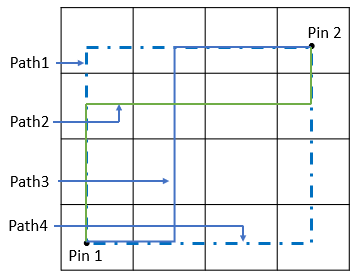
\includegraphics[width=1.5in]{2pinusage}
    \caption{Four possible paths for a two-pin pair.}
    \label{fig:2pinusage}
\end{figure}

If $n$ edges constitute path $i$, and let $M(e)$ be the maximum capacity for edge e, then the total availability $A(i)$ for path $i$ is $A(i)=\sum_{e=0}^{n}M(e)$. Note that for any edge $e$ in path $i$, if $M(e)=0$ then the entire path is eliminated from candidacy. Following the computation of the total availability of each of the potential paths, the probability of each path is calculated. This calculation is done by obtaining the sum of the total availability of all potential paths between the two pins as shown in \Cref{fig:2pinusage}.
If there are k paths, the probability of path $p(i)=\frac{A(i)}{\sum^{k}A}$

Each edge $j$ in path $i$ is assigned a probability $p(i)$ which reflects its likelihood for being used in global routing. Since an edge can belong to more than one potential path, the usage assigned to each edge is a sum of all the path probabilities of which this chosen edge is a part of. Thus, we acquire probabilistic information for each edge to be used in global routing. In an edge-based analyses, this feature provides us valuable information for the routing probability of an edge from a standalone perspective.

\begin{figure}[tb!]
    \centerline{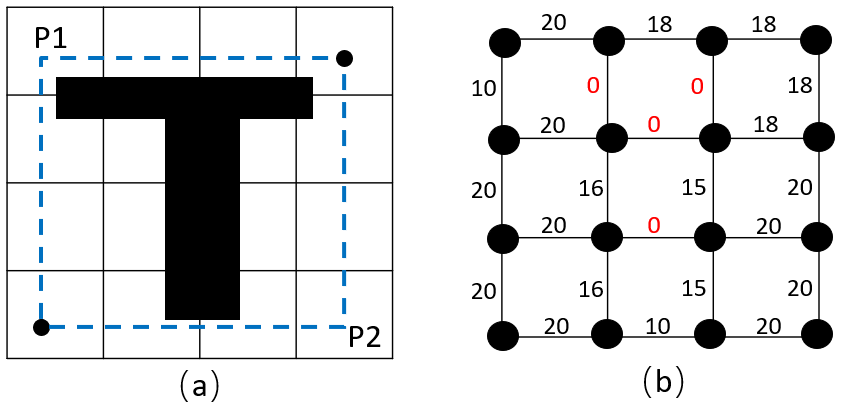
\includegraphics[width=2.6in]{2pinexample}}
    \caption{(a) A design grid with blockage and two possible paths; (b) Corresponding routing graph and related edge capacity.}
    \label{fig:2pinexample}
\end{figure}
An simple example is shown in \Cref{fig:2pinexample}, there are two possible paths, P1 and P2, for routing the pin-pair, where two pins are located at the lower left and upper right corners. From the routing graph we obtain $A(p1)=106$ and $A(p2)=108$. So the probability of choosing path P1 is $p(P1)=106/(106+108)=0.49$, therefore $p(p2)=0.51$. The final usage assigned for edges passed by these two paths will then be increase either 0.49 or 0.51, accordingly.
\end{itemize}

\subsection{Routability-Driven Edge Shifting}
We use our routability information to guide the edge shifting technique in FLUTE\cite{fastroute}. The congestion map heavily affects the structure of Steiner tree hence the actual routing. Therefore, the quality of the congestion map directly affects that of the tree topology.

To perform shifting is to move Steiner points. The edge that connects at least one Steiner point is selected. The moving direction for the Steiner point is perpendicular to the edge, and the allowed range for moving the said Steiner point is determined by all other pins and points that also connect to the two endpoints of the shifting edge, whichever is shorter. As is demonstrated in \Cref{fig:edgeshifting}, the shifting edge is horizontal, the Steiner point is moving in a vertical direction, and the range of moving is determined by the shortest path which previously connected the pin of the shifting edge and another pin. 
\begin{figure}[htbp]
    \centerline{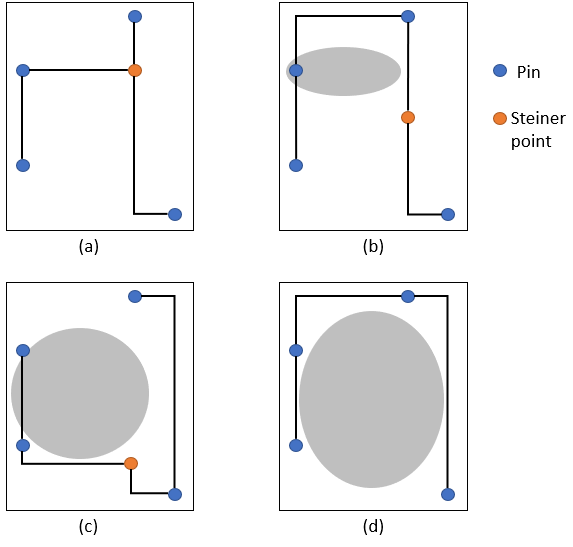
\includegraphics[height=1.8in, width=2.7in]{edgeshifting}}
    \caption{(a) The initial Steiner tree (b) Allowed moving area for Steiner point (c)(d) Modified tree structures based on different congestion map.}
    \label{fig:edgeshifting}
\end{figure}

\subsection{Prediction Model Embedded Routability Optimization}
After the features are extracted, we use MARS \cite{MARS} to predict routability. The reasons of selecting MARS are as follows: 1) Interactions between independent parameters can be captured. 2) Non-linearity can be modeled. 3) Tunning is easy, and in most cases, not needed. 

We pick a median-size design and extract corresponding features.
After a model is trained, we select as testing data three other designs with respective small median and large size.
A model is deemed acceptable if its max-min congestion range of prediction is within 15\% comparing with that of actual.
Then, the congestion model is integrated into the global router, as is shown in \Cref{alg:route}.
After necessary initialisation such as reading design and creating routing graph, initial Steiner trees are constructed for each net by using FLUTE \cite{FLUTE} (line \ref*{alg:ln:flute}).
The congestion map is generated by our model and assigned to each edge of the graph (line \ref*{alg:ln:cong}).
Shifting lines for each Steiner point is determined as the first step of edge shifting,
along which the Steiner point moves to find the least congested spot to optimise the tree structure (line \ref*{alg:ln:es}).
After the Steiner tree is adjusted and the routing topology is conducted, the routing follows (line \ref*{alg:ln:routing}).
The router starts from each optimised tree of nets, and choose the best path candidate based on the congestion map, and finally construct a fully routed design layout.
Once the routing is finished, the actual congestion is produced by real routing path
. Congestion map which previously read from model is then removed (line \ref*{alg:ln:rmcong}), to avoid interference between two kinds of information, predicted and actual, in the final stage.
A Rip-up \& Reroute is performed at last while judging the threshold at each iteration (line \ref*{alg:ln:rrr}).


\begin{algorithm}
    \caption{Routability Model Guided Routing}
    \label{alg:route}
    \begin{algorithmic}[1]
        \Require Placed netlist.
        \State \texttt{Init()};
        \While{net $\gets$ nets.\texttt{read}()}
            \State \texttt{FLUTE}(net); \label{alg:ln:flute}
            \State congestion $\gets$ \texttt{inputGuide}(model); \label{alg:ln:cong}
            \State \texttt{edgeShifting}(net, congestion); \label{alg:ln:es}
            \State \texttt{routing}(net, congestion); \label{alg:ln:routing}
            \State \texttt{removeGuide}(congestion); \label{alg:ln:rmcong}
            \While{FALSE == \texttt{metThreshold}()}
                \State \texttt{ripUpReroute}(); \label{alg:ln:rrr}
            \EndWhile
        \EndWhile
    \end{algorithmic}
\end{algorithm}

% \iffalse
% \begin{algorithm}
% \SetAlgoLined
% \KwResult{Global Routing Instance}
%  initialisation()\;
%  \While{net = nets.read()}{
%     FLUTE(net)\;
%     congestion = inputGuide(model)\;
%     edgeShifting(net, congestion)\;
%     routing(net, congestion)\;
%     removeGuide(congestion)\;
    
%     \While{!metThreshold()}{
%         ripUpReroute()\;
%         }
  
%  }
%  \caption{routability model guided routing}
% \end{algorithm}
% \fi
